\documentclass[9pt]{beamer}\usepackage[]{graphicx}\usepackage[]{color}
%% maxwidth is the original width if it is less than linewidth
%% otherwise use linewidth (to make sure the graphics do not exceed the margin)
\makeatletter
\def\maxwidth{ %
  \ifdim\Gin@nat@width>\linewidth
    \linewidth
  \else
    \Gin@nat@width
  \fi
}
\makeatother

\usepackage{Sweavel}



% Presento style file
\usepackage{config/presento}

% custom command and packages
% custom packages
\usepackage{textpos}
\setlength{\TPHorizModule}{1cm}
\setlength{\TPVertModule}{1cm}

\newcommand\crule[1][black]{\textcolor{#1}{\rule{2cm}{2cm}}}


\usepackage{listings}

\usepackage{amsopn} %eps stuff
\usepackage[dvips]{epsfig} %eps stuff
\usepackage[utf8]{inputenc}
\usepackage[sc]{mathpazo}



\usepackage[sc]{mathpazo}
\linespread{1.05}         % Palladio needs more leading (space between lines)
\usepackage[T1]{fontenc}

\usepackage{cmap}
\usepackage{mathdots}
\usepackage{microtype}
\usepackage[noadjust]{cite}
\usepackage{ulem}
\usepackage{lipsum}
\usepackage{enumerate}
\usepackage{multicol}
\usepackage{amsthm}
\usepackage{enumitem}
\usepackage{graphicx}






% Information
\title{Home Work 4 - Problem 5}
\subtitle{Algorithms}
\author{Rory Flynn, Balaviknesh Sekar}
\institute{University of Colorado Denver}
\date{\today}


\begin{document}

% Title page
\begin{frame}[plain]
\maketitle
\end{frame}





\begin{frame}[fragile]{Home Work 4: Problem 5: Thickness}
     Let $G$ be a simple undirected graph with n vertices labeled $1,2,. . .,n$. The graph $G[r_1 , r_2 , . . . , r_n ]$ is the graph obtained from G by replacing vertex $i$ with $K_{r_i}$ and connecting all possible vertices in neighboring complete graphs. So, for example, $G[1, 1, . . . , 1] = G$, $K_2 [2, 2] = K_4$ , $K_2 [m, n] = K_{m+n}$ , and $K_1 [n] = K_n$.
   
  Using R and igraph:
\begin{Schunk}
\begin{Sinput}
g <- make_empty_graph(directed=F ) +
  vertices(1:3) +
  edge( c(1:3,1:3))
  plot(g)
\end{Sinput}

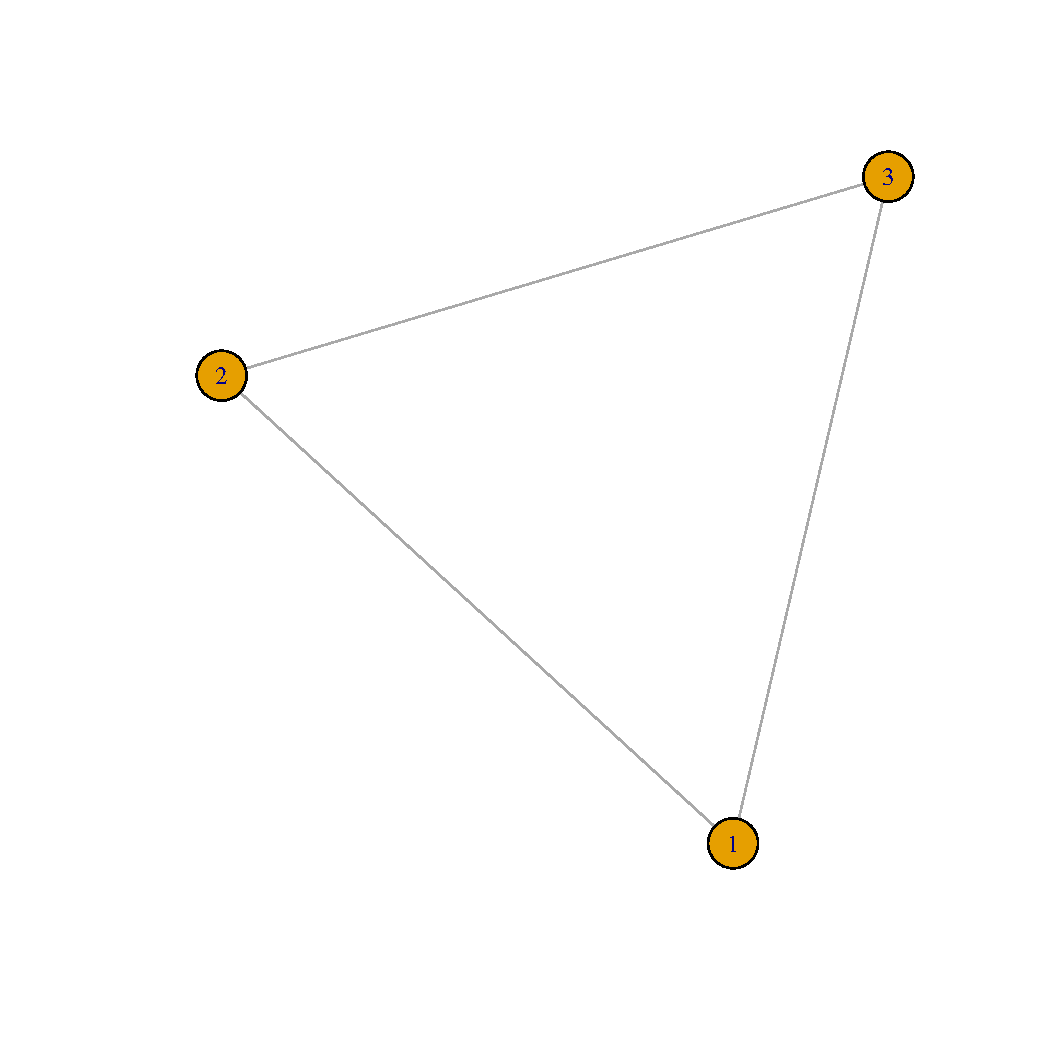
\includegraphics[width=3cm]{figure/unnamed-chunk-1-1} \end{Schunk}
  
\end{frame}

\section{Section no. 1}
\begin{frame}{Part a }
    \begin{problem}
    The independence number $\alpha(G)$ of a graph $G$ is the size of the largest set of independent (mutually nonadjacent) vertices in G. Prove that $\chi(G) \ge \frac{|V (G)|}{\alpha(G)}$.
     \end{problem}
    \begin{proof}
        Let $a_1$ be the largest set of independent (mutually nonadjacent) vertices in G.

        Then there is a set $!a_1$ the members of which are by definition not in $a_1$ but are agent to a member of $a_1$.

        The set $!a_1$ can be sub divided in to set of independent vertices none of wich can be lager than $a_1$ or smaller than 1.

        It fallows that the maximum number of subsets is then $\frac{|V (G)|}{\alpha(G)}$.

        Note that for a correct coloring all members of an independent set can share one color(they are not adjacent), no two sets can share a color however (their nodes are adjacent).

        Thus the chromatic number must be greater or equal the number of independent sub sets.

        Therefore $\chi(G) \ge \frac{|V (G)|}{\alpha(G)}$.
    \end{proof}
\end{frame}

\section{Section no. 2}
\frame{\frametitle{Part b}
    If $G$ is a graph with $n$ vertices, prove that $\alpha(G) = \alpha(G[r_1 , r_2, ... , r_n])$, where each $r_i \in N$.
    \begin{proof}

    \end{proof}

}

\frame{\frametitle{Part c}
    Find both the chromatic number and thickness of $C_3 [2, 2, 2]$ and prove that your answers are correct.
}

\frame{\frametitle{Part d}
    Find both the chromatic number and thickness of $C_5 [2, 2, 2, 2, 2]$ and prove that your answers are correct.
}

\frame{\frametitle{Part e}
    Find both the chromatic number and thickness of $C_n [2, 2, . . . , 2]$ and prove that your answers are correct.
}

\frame{\frametitle{Part f}
    Find both the chromatic number and thickness of $C_5 [3, 3, 3, 3, 3]$ and prove that your answers are correct.
}

\frame{\frametitle{Part g}
    Find both the chromatic number and thickness of $C_5 [4, 4, 4, 4, 3]$ and prove that your answers are correct.
}

\frame{\frametitle{Part h}
    Find both the chromatic number and thickness of $C_7 [4, 4, 4, 4, 4, 4, 4]$ and prove that your answers are correct.
}


\end{document}
